\scanpage{3}
\begin{center}( 2 )\end{center}

Soient $A$ un anneau local noethérien et $\widehat A$ son complété. On a :

\textsc{Lemme.} --- \textit{Le noyau de l'application canonique : $\widehat A\otimes_A D(A)\to D(\widehat A)$ est contenu dans l'intersection : $\displaystyle\bigcap_{M\in\sigma}\left(\widehat A\otimes_A M\right)$, où $\sigma$ désigne l'ensemble des sous-modules $M$ de $D(A)$ tels que $F=D(A)/M$ soit un $A$-module de type fini.}

De ce lemme on déduit que si $D(A)$ est semi-fini au sens de Suzuki \textsuperscript{(10)}, c'est-à-dire somme directe d'un module libre et d'un module de type fini, la suite canonique
\diagram{\begin{tikzcd}[ampersand replacement=\&]
0\arrow[r]\&\widehat A\otimes_A D(A)\arrow[r]\&(\widehat A)\arrow[r]\&D_A(\widehat A)\arrow[r]\&0
\end{tikzcd}}
est exacte.

Cela entraîne notamment :

\textsc{Proposition 4.} --- \textit{Si $A$ est une localité analytiquement \uline{intègre}, $K_{\widehat A}$ est séparable sur $K_A$.}

De même (\textit{cf.} cor. 1 de la prop. 1), si $A$ est un anneau de séries convergentes sur un corps valué complet de caractéristique $p>0$ et tel que $(k:k^p)<+\infty$, $K_{\widehat A}$ est séparable sur $K_A$. Ceci permet de combler ce qui nous paraît être une lacune dans la démonstration donnée par Lang \textsuperscript{(4)} du résultat suivant :

\textsc{Proposition 5.} --- \textit{Si $A=k\{T\}$ est l'anneau des séries convergentes sur un corps $k$ valué complet et algébriquement clos, $K_A$ est quasialgébriquement clos $(C^1)$.}

Un cas particulier de la proposition 4, classique, est que $K((X_1,X_2,\ldots,X_n))$ est séparable sur $K(X_1,\ldots,X_n)$ pour tout corps $K$. Il implique, en tenant compte du théorème de structure de Cohen :

\textsc{Proposition 6.} --- \textit{Soit $A$ un anneau local régulier contenant un corps $k$ tel que $L_A$ soit séparable sur $k$. Alors $K_A$ est aussi séparable sur $k$.}
\margin{\figure{\begin{tikzpicture}[y=1cm]\draw (0,5.8)--(0.2,5.85)--(0,0.05)--(-0.2,0);\node[right] at (0.4,3.4) {\unsure{connu}};\end{tikzpicture}}}

3. \textsc{Critère de réduction analytique.} --- La comparaison de la proposition 1 et des énoncés de Suzuki et Mount suggère l'existence d'un critère de réduction analytique sous-jacent; nous nous proposons de voir dans ce paragraphe comment les conclusions du paragraphe 2 permettent d'en obtenir un. Notons tout d'abord le lemme suivant qui peut être considéré comme classique :

\textsc{Lemme.} --- \textit{Soit $A$ un anneau local noethérien analytiquement intègre et tel que $K_{\widehat A}$ soit séparable sur $K_A$. Si $B$ est un anneau local intègre de la forme $B=C_{\mathfrak p}$, où $C$ est une $A$-algèbre \uline{finie} et $\mathfrak p$ un idéal premier de $C$ tel que $\mathfrak p\cap A=\mathfrak M$ ($\mathfrak M$ idéal maximal de $A$), $B$ est analytiquement réduit.}
\margin{\unsure{faux si on ne suppose pas} $A\to B$ \unsure{injectif} ??}

On en déduit :

\textsc{Théorème.} --- \textit{Soit $A$ un anneau local régulier vérifiant l'une ou l'autre des conditions suivantes :}

$(h_1)$ \textit{$K_A$ est de caractéristique $0$;}

$(h_2)$ \figure{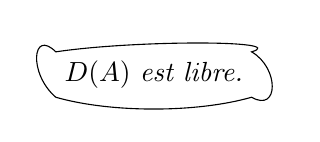
\begin{tikzpicture}[baseline=(t.base)]\node[inner sep=3pt] (t) {$D(A)$ \textit{est libre.}};\draw (t.south west) .. controls +(-0.35,0.3) and +(-0.3,0.3) .. (t.north west) .. controls +(1,0.15) and +(0.5,0.15) .. (t.north east) .. controls +(0.35,-0.2) and +(0.35,-0.2) .. (t.south east) .. controls +(-0.7,-0.2) and +(0.7,-0.2) .. (t.south west);\end{tikzpicture}}

\mspage{2}
